% Convert with command:
% convert -density 300 pic.pdf -quality 100 pic.png
\documentclass[crop,tikz,border=0pt]{standalone}
\usetikzlibrary{arrows.meta}
\usetikzlibrary{calc}
\usetikzlibrary{snakes}
\usetikzlibrary{shapes.geometric}
\begin{document}
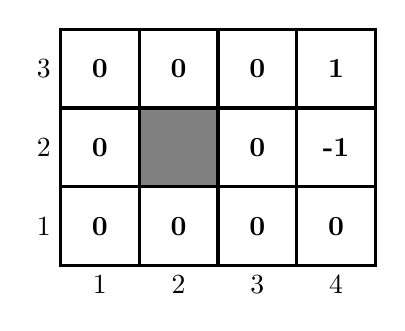
\begin{tikzpicture}
% apply \usetikzlibrary{calc} when importing this file with \input

% https://tex.stackexchange.com/questions/45808/tikz-grid-lines
% #1 size of grid
% Example: \grid{4}
\newcommand{\grid}[1] {
  \newcommand*{\size}{#1}
  \newcommand*{\xMin}{0}%
  \newcommand*{\xMax}{\size}%
  \newcommand*{\yMin}{0}%
  \newcommand*{\yMax}{\size}%
  % Vertical lines
  \foreach \i[evaluate=\i as \n using int(\i+1)] in {\xMin,...,\xMax} {
      \draw [very thick,black,fill=black!20!white] (\i,\yMin) -- (\i,\yMax);
      \ifnum \i < \size
          \node [below] at (\i + 1 / 2,\yMin) {$\n$};
      \fi
  }
  % Horizontal lines
  \foreach \i[evaluate=\i as \n using int(\i+1)] in {\yMin,...,\yMax} {
      \draw [very thick,black] (\xMin,\i) -- (\xMax,\i);
      \ifnum \i < \size
          \node [left] at (\xMin,\i + 1 / 2) {$\n$};
      \fi
  }
  % Background image
  \draw [very thick, draw=black, fill=white] (0,0) grid  (\size,\size) rectangle (0,0);
}

% https://tex.stackexchange.com/questions/45808/tikz-grid-lines
% #1 row amount
% #2 col amount
% Example with 2 rows and 3 cols: \grid{2}{3}
\newcommand{\customgrid}[2] {
  \newcommand*{\rows}{#1}%
  \newcommand*{\cols}{#2}%
  \newcommand*{\xMin}{0}%
  \newcommand*{\xMax}{\cols}%
  \newcommand*{\yMin}{0}%
  \newcommand*{\yMax}{\rows}%
  % Vertical lines
  \foreach \i[evaluate=\i as \n using int(\i+1)] in {\xMin,...,\xMax} {
      \draw [very thick,black,fill=black!20!white] (\i,\yMin) -- (\i,\yMax);
      \ifnum \i < \cols
          \node [below] at (\i + 1 / 2,\yMin) {$\n$};
      \fi
  }
  % Horizontal lines
  \foreach \i[evaluate=\i as \n using int(\i+1)] in {\yMin,...,\yMax} {
      \draw [very thick,black] (\xMin,\i) -- (\xMax,\i);
      \ifnum \i < \rows
          \node [left] at (\xMin,\i + 1 / 2) {$\n$};
      \fi
  }
  % Background image
  \draw [very thick, draw=black, fill=white] (0,0) grid  (\cols,\rows) rectangle (0,0);
}

% #1 - coordinates (row, col)
% #2 - text
% Example: \pithole{3, 1}{P}
\newcommand{\pithole}[2] {
  \node at ($($(#1) + (0, 0)$)!0.5!($(#1) + (-1, -1)$)$) [
    shape=circle, draw=blue!, line width=0.5mm, fill=white, text centered, text=blue, font=\bfseries
  ] {#2};
}

% #1 monster coordinates (col, row)
% Example: \monster{2, 3}
\newcommand{\monster}[1] {
  % https://tex.stackexchange.com/questions/398501/tikz-coordinate-addition-in-path
  \node (M) at ($($(#1) + (-1, -1)$)!0.5!($(#1) + (0, 0)$)$) [shape=circle, fill=white, text centered, text=red, font=\bfseries] {W};
}

% #1 gold coordinates (col, row)
% Example: \gold{4, 4}
\newcommand{\gold}[1] {
  \node (M) at ($($(#1) + (-1, -1)$)!0.5!($(#1) + (0, 0)$)$) [
    fill=white, text centered, text={rgb:red,255;green,215;blue,0},, font=\bfseries
  ] {G};
}

% #1 rotation of the figure in degrees, optional: Default: 0
% #2 coordinates on the grid(col, row)
% Example: \human[90]{1, 3}
% Example: \human{1, 3}
\newcommand{\human}[2][0] {
  % https://tex.stackexchange.com/questions/398501/tikz-coordinate-addition-in-path
  % Place the rotation center to the center of the figure
  % (-1, -1) used due to the skew from the user input that goes from (1, 1) to (n, n)
  \begin{scope}[rotate around={#1:($(#2) + (-0.5,-0.5)$)}]
    % head
    \node (A) at ($(#2) + (0.7,0.5) + (-1, -1)$) [
      shape=circle, scale=0.6, fill=white, text centered, draw=black, line width=0.2mm
    ] {};
    % body
    \draw[-] ($(#2) + (0.6,0.5) + (-1, -1)$) -- ($(#2) + (0.3,0.5) + (-1, -1)$) node[] {}; 
    % hands
    \draw[-] ($(#2) + (0.6,0.5) + (-1, -1)$) -- ($(#2) + (0.4,0.4) + (-1, -1)$) node[] {}; 
    \draw[-] ($(#2) + (0.6,0.5) + (-1, -1)$) -- ($(#2) + (0.4,0.6) + (-1, -1)$) node[] {}; 
    % legs
    \draw[-] ($(#2) + (0.3,0.5) + (-1, -1)$) -- ($(#2) + (0.1,0.4) + (-1, -1)$) node[] {}; 
    \draw[-] ($(#2) + (0.3,0.5) + (-1, -1)$) -- ($(#2) + (0.1,0.6) + (-1, -1)$) node[] {}; 
  \end{scope}
}

% #1 coordinates of stench (col, row)
% Example: \stench{1, 3}
\newcommand{\stench}[1] {
  \draw[
    decorate,decoration={snake,amplitude=.4mm,segment length=1mm,post length=0.1mm},black
  ] ($(#1) + (-0.2,-0.5)$) -- ($(#1) + (-0.7,-0.5)$);
  \node at ($(#1) + (-0.5, -0.6)$) [] {\tiny Stench};
}

% #1 coordinates of breeze (col, row)
% Example: \breeze{1, 3}
\newcommand{\breeze}[1] {
  \draw[-,blue] ($(#1) + (0.4,0.4) + (-1, -1)$) -- ($(#1) + (0.5,0.6) + (-1, -1)$) node[] {}; 
  \draw[-,blue] ($(#1) + (0.5,0.6) + (-1, -1)$) -- ($(#1) + (0.6,0.4) + (-1, -1)$) node[] {}; 
  \node at ($(#1) + (0.5,0.35) + (-1, -1)$) [color=blue] {\tiny Breeze};
}

% #1 coordinates of OK word (col, row)
% Example: \ok{1, 3}
\newcommand{\ok}[1] {
  \node (M) at ($($(#1) + (-1, -1.6)$)!0.5!($(#1) + (0, 0)$)$) [fill=white, text centered, text=green, font=\bfseries] {\tiny OK};
}

% #1 coordinates of any word (col, row)
% #2 text itself
% Example: \gridtext{1, 3}{mytext}
\newcommand{\gridtext}[2] {
  \node (T) at ($($(#1) + (-1, -1)$)!0.5!($(#1) + (0, 0)$)$) [
      text centered, text=black, font=\bfseries
  ] {#2};
}

% #1 coordinates of the square (col, row)
% #2 color of the square
% Example: \squarecolor{2, 2}{green}
\newcommand{\squarecolor}[2] {
  \node (C) at ($(#1) + (-0.5, -0.5)$) [
    shape=rectangle,fill=#2,minimum width=9.5mm,minimum height=9.5mm
  ] {};
}

% #1 rotation of the figure in degrees, optional: Default: 0
% #2 coordinates on the grid(col, row)
% Example: \human[90]{1, 3}
% Example: \human{1, 3}
\newcommand{\arrow}[2][0] {
  % https://tex.stackexchange.com/questions/398501/tikz-coordinate-addition-in-path
  % Place the rotation center to the center of the figure
  % (-1, -1) used due to the skew from the user input that goes from (1, 1) to (n, n)
  \begin{scope}[rotate around={#1:($(#2) + (-0.5,-0.5)$)}]
    % head
    \node (A) at ($(#2) + (0.6,0.5) + (-1, -1)$) [
      shape=isosceles triangle, rotate=#1, scale=0.6,
      fill=black, text centered, draw=black, line width=0.1mm
    ] {};
    % body
    \draw[-] ($(#2) + (0.6,0.5) + (-1, -1)$) -- ($(#2) + (0.3,0.5) + (-1, -1)$) node[] {}; 
  \end{scope}
}

\customgrid{3}{4}

\gridtext{4, 2}{-1}

\gridtext{4, 3}{1}

\squarecolor{2, 2}{gray}

\gridtext{1, 1}{0}
\gridtext{1, 2}{0}
\gridtext{1, 3}{0}

\gridtext{2, 1}{0}
\gridtext{2, 3}{0}

\gridtext{3, 1}{0}
\gridtext{3, 2}{0}
\gridtext{3, 3}{0}

\gridtext{4, 1}{0}

% \foreach \x in {1,...,4} 
%     \foreach \y in {1,..., 3} {
%         \gridtext{\x, \y}{0};
%     }

\end{tikzpicture}

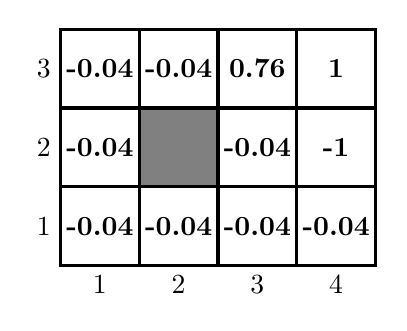
\begin{tikzpicture}
% apply \usetikzlibrary{calc} when importing this file with \input

% https://tex.stackexchange.com/questions/45808/tikz-grid-lines
% #1 size of grid
% Example: \grid{4}
\newcommand{\grid}[1] {
  \newcommand*{\size}{#1}
  \newcommand*{\xMin}{0}%
  \newcommand*{\xMax}{\size}%
  \newcommand*{\yMin}{0}%
  \newcommand*{\yMax}{\size}%
  % Vertical lines
  \foreach \i[evaluate=\i as \n using int(\i+1)] in {\xMin,...,\xMax} {
      \draw [very thick,black,fill=black!20!white] (\i,\yMin) -- (\i,\yMax);
      \ifnum \i < \size
          \node [below] at (\i + 1 / 2,\yMin) {$\n$};
      \fi
  }
  % Horizontal lines
  \foreach \i[evaluate=\i as \n using int(\i+1)] in {\yMin,...,\yMax} {
      \draw [very thick,black] (\xMin,\i) -- (\xMax,\i);
      \ifnum \i < \size
          \node [left] at (\xMin,\i + 1 / 2) {$\n$};
      \fi
  }
  % Background image
  \draw [very thick, draw=black, fill=white] (0,0) grid  (\size,\size) rectangle (0,0);
}

% https://tex.stackexchange.com/questions/45808/tikz-grid-lines
% #1 row amount
% #2 col amount
% Example with 2 rows and 3 cols: \grid{2}{3}
\newcommand{\customgrid}[2] {
  \newcommand*{\rows}{#1}%
  \newcommand*{\cols}{#2}%
  \newcommand*{\xMin}{0}%
  \newcommand*{\xMax}{\cols}%
  \newcommand*{\yMin}{0}%
  \newcommand*{\yMax}{\rows}%
  % Vertical lines
  \foreach \i[evaluate=\i as \n using int(\i+1)] in {\xMin,...,\xMax} {
      \draw [very thick,black,fill=black!20!white] (\i,\yMin) -- (\i,\yMax);
      \ifnum \i < \cols
          \node [below] at (\i + 1 / 2,\yMin) {$\n$};
      \fi
  }
  % Horizontal lines
  \foreach \i[evaluate=\i as \n using int(\i+1)] in {\yMin,...,\yMax} {
      \draw [very thick,black] (\xMin,\i) -- (\xMax,\i);
      \ifnum \i < \rows
          \node [left] at (\xMin,\i + 1 / 2) {$\n$};
      \fi
  }
  % Background image
  \draw [very thick, draw=black, fill=white] (0,0) grid  (\cols,\rows) rectangle (0,0);
}

% #1 - coordinates (row, col)
% #2 - text
% Example: \pithole{3, 1}{P}
\newcommand{\pithole}[2] {
  \node at ($($(#1) + (0, 0)$)!0.5!($(#1) + (-1, -1)$)$) [
    shape=circle, draw=blue!, line width=0.5mm, fill=white, text centered, text=blue, font=\bfseries
  ] {#2};
}

% #1 monster coordinates (col, row)
% Example: \monster{2, 3}
\newcommand{\monster}[1] {
  % https://tex.stackexchange.com/questions/398501/tikz-coordinate-addition-in-path
  \node (M) at ($($(#1) + (-1, -1)$)!0.5!($(#1) + (0, 0)$)$) [shape=circle, fill=white, text centered, text=red, font=\bfseries] {W};
}

% #1 gold coordinates (col, row)
% Example: \gold{4, 4}
\newcommand{\gold}[1] {
  \node (M) at ($($(#1) + (-1, -1)$)!0.5!($(#1) + (0, 0)$)$) [
    fill=white, text centered, text={rgb:red,255;green,215;blue,0},, font=\bfseries
  ] {G};
}

% #1 rotation of the figure in degrees, optional: Default: 0
% #2 coordinates on the grid(col, row)
% Example: \human[90]{1, 3}
% Example: \human{1, 3}
\newcommand{\human}[2][0] {
  % https://tex.stackexchange.com/questions/398501/tikz-coordinate-addition-in-path
  % Place the rotation center to the center of the figure
  % (-1, -1) used due to the skew from the user input that goes from (1, 1) to (n, n)
  \begin{scope}[rotate around={#1:($(#2) + (-0.5,-0.5)$)}]
    % head
    \node (A) at ($(#2) + (0.7,0.5) + (-1, -1)$) [
      shape=circle, scale=0.6, fill=white, text centered, draw=black, line width=0.2mm
    ] {};
    % body
    \draw[-] ($(#2) + (0.6,0.5) + (-1, -1)$) -- ($(#2) + (0.3,0.5) + (-1, -1)$) node[] {}; 
    % hands
    \draw[-] ($(#2) + (0.6,0.5) + (-1, -1)$) -- ($(#2) + (0.4,0.4) + (-1, -1)$) node[] {}; 
    \draw[-] ($(#2) + (0.6,0.5) + (-1, -1)$) -- ($(#2) + (0.4,0.6) + (-1, -1)$) node[] {}; 
    % legs
    \draw[-] ($(#2) + (0.3,0.5) + (-1, -1)$) -- ($(#2) + (0.1,0.4) + (-1, -1)$) node[] {}; 
    \draw[-] ($(#2) + (0.3,0.5) + (-1, -1)$) -- ($(#2) + (0.1,0.6) + (-1, -1)$) node[] {}; 
  \end{scope}
}

% #1 coordinates of stench (col, row)
% Example: \stench{1, 3}
\newcommand{\stench}[1] {
  \draw[
    decorate,decoration={snake,amplitude=.4mm,segment length=1mm,post length=0.1mm},black
  ] ($(#1) + (-0.2,-0.5)$) -- ($(#1) + (-0.7,-0.5)$);
  \node at ($(#1) + (-0.5, -0.6)$) [] {\tiny Stench};
}

% #1 coordinates of breeze (col, row)
% Example: \breeze{1, 3}
\newcommand{\breeze}[1] {
  \draw[-,blue] ($(#1) + (0.4,0.4) + (-1, -1)$) -- ($(#1) + (0.5,0.6) + (-1, -1)$) node[] {}; 
  \draw[-,blue] ($(#1) + (0.5,0.6) + (-1, -1)$) -- ($(#1) + (0.6,0.4) + (-1, -1)$) node[] {}; 
  \node at ($(#1) + (0.5,0.35) + (-1, -1)$) [color=blue] {\tiny Breeze};
}

% #1 coordinates of OK word (col, row)
% Example: \ok{1, 3}
\newcommand{\ok}[1] {
  \node (M) at ($($(#1) + (-1, -1.6)$)!0.5!($(#1) + (0, 0)$)$) [fill=white, text centered, text=green, font=\bfseries] {\tiny OK};
}

% #1 coordinates of any word (col, row)
% #2 text itself
% Example: \gridtext{1, 3}{mytext}
\newcommand{\gridtext}[2] {
  \node (T) at ($($(#1) + (-1, -1)$)!0.5!($(#1) + (0, 0)$)$) [
      text centered, text=black, font=\bfseries
  ] {#2};
}

% #1 coordinates of the square (col, row)
% #2 color of the square
% Example: \squarecolor{2, 2}{green}
\newcommand{\squarecolor}[2] {
  \node (C) at ($(#1) + (-0.5, -0.5)$) [
    shape=rectangle,fill=#2,minimum width=9.5mm,minimum height=9.5mm
  ] {};
}

% #1 rotation of the figure in degrees, optional: Default: 0
% #2 coordinates on the grid(col, row)
% Example: \human[90]{1, 3}
% Example: \human{1, 3}
\newcommand{\arrow}[2][0] {
  % https://tex.stackexchange.com/questions/398501/tikz-coordinate-addition-in-path
  % Place the rotation center to the center of the figure
  % (-1, -1) used due to the skew from the user input that goes from (1, 1) to (n, n)
  \begin{scope}[rotate around={#1:($(#2) + (-0.5,-0.5)$)}]
    % head
    \node (A) at ($(#2) + (0.6,0.5) + (-1, -1)$) [
      shape=isosceles triangle, rotate=#1, scale=0.6,
      fill=black, text centered, draw=black, line width=0.1mm
    ] {};
    % body
    \draw[-] ($(#2) + (0.6,0.5) + (-1, -1)$) -- ($(#2) + (0.3,0.5) + (-1, -1)$) node[] {}; 
  \end{scope}
}

\customgrid{3}{4}

\gridtext{4, 2}{-1}

\gridtext{4, 3}{1}

\squarecolor{2, 2}{gray}

\gridtext{1, 1}{-0.04}
\gridtext{1, 2}{-0.04}
\gridtext{1, 3}{-0.04}

\gridtext{2, 1}{-0.04}
\gridtext{2, 3}{-0.04}

\gridtext{3, 1}{-0.04}
\gridtext{3, 2}{-0.04}
\gridtext{3, 3}{0.76}

\gridtext{4, 1}{-0.04}

\end{tikzpicture}

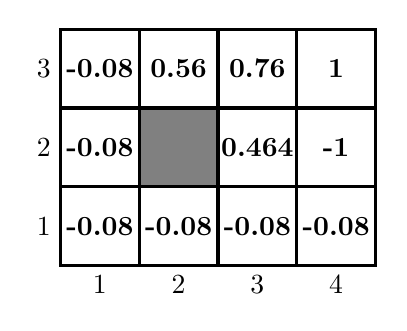
\begin{tikzpicture}
% apply \usetikzlibrary{calc} when importing this file with \input

% https://tex.stackexchange.com/questions/45808/tikz-grid-lines
% #1 size of grid
% Example: \grid{4}
\newcommand{\grid}[1] {
  \newcommand*{\size}{#1}
  \newcommand*{\xMin}{0}%
  \newcommand*{\xMax}{\size}%
  \newcommand*{\yMin}{0}%
  \newcommand*{\yMax}{\size}%
  % Vertical lines
  \foreach \i[evaluate=\i as \n using int(\i+1)] in {\xMin,...,\xMax} {
      \draw [very thick,black,fill=black!20!white] (\i,\yMin) -- (\i,\yMax);
      \ifnum \i < \size
          \node [below] at (\i + 1 / 2,\yMin) {$\n$};
      \fi
  }
  % Horizontal lines
  \foreach \i[evaluate=\i as \n using int(\i+1)] in {\yMin,...,\yMax} {
      \draw [very thick,black] (\xMin,\i) -- (\xMax,\i);
      \ifnum \i < \size
          \node [left] at (\xMin,\i + 1 / 2) {$\n$};
      \fi
  }
  % Background image
  \draw [very thick, draw=black, fill=white] (0,0) grid  (\size,\size) rectangle (0,0);
}

% https://tex.stackexchange.com/questions/45808/tikz-grid-lines
% #1 row amount
% #2 col amount
% Example with 2 rows and 3 cols: \grid{2}{3}
\newcommand{\customgrid}[2] {
  \newcommand*{\rows}{#1}%
  \newcommand*{\cols}{#2}%
  \newcommand*{\xMin}{0}%
  \newcommand*{\xMax}{\cols}%
  \newcommand*{\yMin}{0}%
  \newcommand*{\yMax}{\rows}%
  % Vertical lines
  \foreach \i[evaluate=\i as \n using int(\i+1)] in {\xMin,...,\xMax} {
      \draw [very thick,black,fill=black!20!white] (\i,\yMin) -- (\i,\yMax);
      \ifnum \i < \cols
          \node [below] at (\i + 1 / 2,\yMin) {$\n$};
      \fi
  }
  % Horizontal lines
  \foreach \i[evaluate=\i as \n using int(\i+1)] in {\yMin,...,\yMax} {
      \draw [very thick,black] (\xMin,\i) -- (\xMax,\i);
      \ifnum \i < \rows
          \node [left] at (\xMin,\i + 1 / 2) {$\n$};
      \fi
  }
  % Background image
  \draw [very thick, draw=black, fill=white] (0,0) grid  (\cols,\rows) rectangle (0,0);
}

% #1 - coordinates (row, col)
% #2 - text
% Example: \pithole{3, 1}{P}
\newcommand{\pithole}[2] {
  \node at ($($(#1) + (0, 0)$)!0.5!($(#1) + (-1, -1)$)$) [
    shape=circle, draw=blue!, line width=0.5mm, fill=white, text centered, text=blue, font=\bfseries
  ] {#2};
}

% #1 monster coordinates (col, row)
% Example: \monster{2, 3}
\newcommand{\monster}[1] {
  % https://tex.stackexchange.com/questions/398501/tikz-coordinate-addition-in-path
  \node (M) at ($($(#1) + (-1, -1)$)!0.5!($(#1) + (0, 0)$)$) [shape=circle, fill=white, text centered, text=red, font=\bfseries] {W};
}

% #1 gold coordinates (col, row)
% Example: \gold{4, 4}
\newcommand{\gold}[1] {
  \node (M) at ($($(#1) + (-1, -1)$)!0.5!($(#1) + (0, 0)$)$) [
    fill=white, text centered, text={rgb:red,255;green,215;blue,0},, font=\bfseries
  ] {G};
}

% #1 rotation of the figure in degrees, optional: Default: 0
% #2 coordinates on the grid(col, row)
% Example: \human[90]{1, 3}
% Example: \human{1, 3}
\newcommand{\human}[2][0] {
  % https://tex.stackexchange.com/questions/398501/tikz-coordinate-addition-in-path
  % Place the rotation center to the center of the figure
  % (-1, -1) used due to the skew from the user input that goes from (1, 1) to (n, n)
  \begin{scope}[rotate around={#1:($(#2) + (-0.5,-0.5)$)}]
    % head
    \node (A) at ($(#2) + (0.7,0.5) + (-1, -1)$) [
      shape=circle, scale=0.6, fill=white, text centered, draw=black, line width=0.2mm
    ] {};
    % body
    \draw[-] ($(#2) + (0.6,0.5) + (-1, -1)$) -- ($(#2) + (0.3,0.5) + (-1, -1)$) node[] {}; 
    % hands
    \draw[-] ($(#2) + (0.6,0.5) + (-1, -1)$) -- ($(#2) + (0.4,0.4) + (-1, -1)$) node[] {}; 
    \draw[-] ($(#2) + (0.6,0.5) + (-1, -1)$) -- ($(#2) + (0.4,0.6) + (-1, -1)$) node[] {}; 
    % legs
    \draw[-] ($(#2) + (0.3,0.5) + (-1, -1)$) -- ($(#2) + (0.1,0.4) + (-1, -1)$) node[] {}; 
    \draw[-] ($(#2) + (0.3,0.5) + (-1, -1)$) -- ($(#2) + (0.1,0.6) + (-1, -1)$) node[] {}; 
  \end{scope}
}

% #1 coordinates of stench (col, row)
% Example: \stench{1, 3}
\newcommand{\stench}[1] {
  \draw[
    decorate,decoration={snake,amplitude=.4mm,segment length=1mm,post length=0.1mm},black
  ] ($(#1) + (-0.2,-0.5)$) -- ($(#1) + (-0.7,-0.5)$);
  \node at ($(#1) + (-0.5, -0.6)$) [] {\tiny Stench};
}

% #1 coordinates of breeze (col, row)
% Example: \breeze{1, 3}
\newcommand{\breeze}[1] {
  \draw[-,blue] ($(#1) + (0.4,0.4) + (-1, -1)$) -- ($(#1) + (0.5,0.6) + (-1, -1)$) node[] {}; 
  \draw[-,blue] ($(#1) + (0.5,0.6) + (-1, -1)$) -- ($(#1) + (0.6,0.4) + (-1, -1)$) node[] {}; 
  \node at ($(#1) + (0.5,0.35) + (-1, -1)$) [color=blue] {\tiny Breeze};
}

% #1 coordinates of OK word (col, row)
% Example: \ok{1, 3}
\newcommand{\ok}[1] {
  \node (M) at ($($(#1) + (-1, -1.6)$)!0.5!($(#1) + (0, 0)$)$) [fill=white, text centered, text=green, font=\bfseries] {\tiny OK};
}

% #1 coordinates of any word (col, row)
% #2 text itself
% Example: \gridtext{1, 3}{mytext}
\newcommand{\gridtext}[2] {
  \node (T) at ($($(#1) + (-1, -1)$)!0.5!($(#1) + (0, 0)$)$) [
      text centered, text=black, font=\bfseries
  ] {#2};
}

% #1 coordinates of the square (col, row)
% #2 color of the square
% Example: \squarecolor{2, 2}{green}
\newcommand{\squarecolor}[2] {
  \node (C) at ($(#1) + (-0.5, -0.5)$) [
    shape=rectangle,fill=#2,minimum width=9.5mm,minimum height=9.5mm
  ] {};
}

% #1 rotation of the figure in degrees, optional: Default: 0
% #2 coordinates on the grid(col, row)
% Example: \human[90]{1, 3}
% Example: \human{1, 3}
\newcommand{\arrow}[2][0] {
  % https://tex.stackexchange.com/questions/398501/tikz-coordinate-addition-in-path
  % Place the rotation center to the center of the figure
  % (-1, -1) used due to the skew from the user input that goes from (1, 1) to (n, n)
  \begin{scope}[rotate around={#1:($(#2) + (-0.5,-0.5)$)}]
    % head
    \node (A) at ($(#2) + (0.6,0.5) + (-1, -1)$) [
      shape=isosceles triangle, rotate=#1, scale=0.6,
      fill=black, text centered, draw=black, line width=0.1mm
    ] {};
    % body
    \draw[-] ($(#2) + (0.6,0.5) + (-1, -1)$) -- ($(#2) + (0.3,0.5) + (-1, -1)$) node[] {}; 
  \end{scope}
}

\customgrid{3}{4}

\gridtext{4, 2}{-1}

\gridtext{4, 3}{1}

\squarecolor{2, 2}{gray}

\gridtext{1, 1}{-0.08}
\gridtext{1, 2}{-0.08}
\gridtext{1, 3}{-0.08}

\gridtext{2, 1}{-0.08}
\gridtext{2, 3}{0.56}

\gridtext{3, 1}{-0.08}
\gridtext{3, 2}{0.464}
\gridtext{3, 3}{0.76}

\gridtext{4, 1}{-0.08}

\end{tikzpicture}

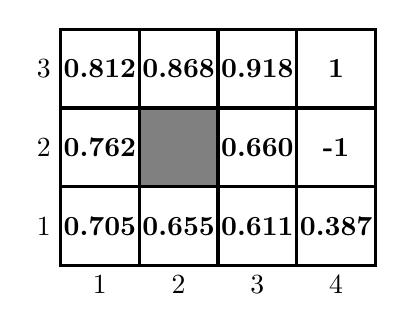
\begin{tikzpicture}
% apply \usetikzlibrary{calc} when importing this file with \input

% https://tex.stackexchange.com/questions/45808/tikz-grid-lines
% #1 size of grid
% Example: \grid{4}
\newcommand{\grid}[1] {
  \newcommand*{\size}{#1}
  \newcommand*{\xMin}{0}%
  \newcommand*{\xMax}{\size}%
  \newcommand*{\yMin}{0}%
  \newcommand*{\yMax}{\size}%
  % Vertical lines
  \foreach \i[evaluate=\i as \n using int(\i+1)] in {\xMin,...,\xMax} {
      \draw [very thick,black,fill=black!20!white] (\i,\yMin) -- (\i,\yMax);
      \ifnum \i < \size
          \node [below] at (\i + 1 / 2,\yMin) {$\n$};
      \fi
  }
  % Horizontal lines
  \foreach \i[evaluate=\i as \n using int(\i+1)] in {\yMin,...,\yMax} {
      \draw [very thick,black] (\xMin,\i) -- (\xMax,\i);
      \ifnum \i < \size
          \node [left] at (\xMin,\i + 1 / 2) {$\n$};
      \fi
  }
  % Background image
  \draw [very thick, draw=black, fill=white] (0,0) grid  (\size,\size) rectangle (0,0);
}

% https://tex.stackexchange.com/questions/45808/tikz-grid-lines
% #1 row amount
% #2 col amount
% Example with 2 rows and 3 cols: \grid{2}{3}
\newcommand{\customgrid}[2] {
  \newcommand*{\rows}{#1}%
  \newcommand*{\cols}{#2}%
  \newcommand*{\xMin}{0}%
  \newcommand*{\xMax}{\cols}%
  \newcommand*{\yMin}{0}%
  \newcommand*{\yMax}{\rows}%
  % Vertical lines
  \foreach \i[evaluate=\i as \n using int(\i+1)] in {\xMin,...,\xMax} {
      \draw [very thick,black,fill=black!20!white] (\i,\yMin) -- (\i,\yMax);
      \ifnum \i < \cols
          \node [below] at (\i + 1 / 2,\yMin) {$\n$};
      \fi
  }
  % Horizontal lines
  \foreach \i[evaluate=\i as \n using int(\i+1)] in {\yMin,...,\yMax} {
      \draw [very thick,black] (\xMin,\i) -- (\xMax,\i);
      \ifnum \i < \rows
          \node [left] at (\xMin,\i + 1 / 2) {$\n$};
      \fi
  }
  % Background image
  \draw [very thick, draw=black, fill=white] (0,0) grid  (\cols,\rows) rectangle (0,0);
}

% #1 - coordinates (row, col)
% #2 - text
% Example: \pithole{3, 1}{P}
\newcommand{\pithole}[2] {
  \node at ($($(#1) + (0, 0)$)!0.5!($(#1) + (-1, -1)$)$) [
    shape=circle, draw=blue!, line width=0.5mm, fill=white, text centered, text=blue, font=\bfseries
  ] {#2};
}

% #1 monster coordinates (col, row)
% Example: \monster{2, 3}
\newcommand{\monster}[1] {
  % https://tex.stackexchange.com/questions/398501/tikz-coordinate-addition-in-path
  \node (M) at ($($(#1) + (-1, -1)$)!0.5!($(#1) + (0, 0)$)$) [shape=circle, fill=white, text centered, text=red, font=\bfseries] {W};
}

% #1 gold coordinates (col, row)
% Example: \gold{4, 4}
\newcommand{\gold}[1] {
  \node (M) at ($($(#1) + (-1, -1)$)!0.5!($(#1) + (0, 0)$)$) [
    fill=white, text centered, text={rgb:red,255;green,215;blue,0},, font=\bfseries
  ] {G};
}

% #1 rotation of the figure in degrees, optional: Default: 0
% #2 coordinates on the grid(col, row)
% Example: \human[90]{1, 3}
% Example: \human{1, 3}
\newcommand{\human}[2][0] {
  % https://tex.stackexchange.com/questions/398501/tikz-coordinate-addition-in-path
  % Place the rotation center to the center of the figure
  % (-1, -1) used due to the skew from the user input that goes from (1, 1) to (n, n)
  \begin{scope}[rotate around={#1:($(#2) + (-0.5,-0.5)$)}]
    % head
    \node (A) at ($(#2) + (0.7,0.5) + (-1, -1)$) [
      shape=circle, scale=0.6, fill=white, text centered, draw=black, line width=0.2mm
    ] {};
    % body
    \draw[-] ($(#2) + (0.6,0.5) + (-1, -1)$) -- ($(#2) + (0.3,0.5) + (-1, -1)$) node[] {}; 
    % hands
    \draw[-] ($(#2) + (0.6,0.5) + (-1, -1)$) -- ($(#2) + (0.4,0.4) + (-1, -1)$) node[] {}; 
    \draw[-] ($(#2) + (0.6,0.5) + (-1, -1)$) -- ($(#2) + (0.4,0.6) + (-1, -1)$) node[] {}; 
    % legs
    \draw[-] ($(#2) + (0.3,0.5) + (-1, -1)$) -- ($(#2) + (0.1,0.4) + (-1, -1)$) node[] {}; 
    \draw[-] ($(#2) + (0.3,0.5) + (-1, -1)$) -- ($(#2) + (0.1,0.6) + (-1, -1)$) node[] {}; 
  \end{scope}
}

% #1 coordinates of stench (col, row)
% Example: \stench{1, 3}
\newcommand{\stench}[1] {
  \draw[
    decorate,decoration={snake,amplitude=.4mm,segment length=1mm,post length=0.1mm},black
  ] ($(#1) + (-0.2,-0.5)$) -- ($(#1) + (-0.7,-0.5)$);
  \node at ($(#1) + (-0.5, -0.6)$) [] {\tiny Stench};
}

% #1 coordinates of breeze (col, row)
% Example: \breeze{1, 3}
\newcommand{\breeze}[1] {
  \draw[-,blue] ($(#1) + (0.4,0.4) + (-1, -1)$) -- ($(#1) + (0.5,0.6) + (-1, -1)$) node[] {}; 
  \draw[-,blue] ($(#1) + (0.5,0.6) + (-1, -1)$) -- ($(#1) + (0.6,0.4) + (-1, -1)$) node[] {}; 
  \node at ($(#1) + (0.5,0.35) + (-1, -1)$) [color=blue] {\tiny Breeze};
}

% #1 coordinates of OK word (col, row)
% Example: \ok{1, 3}
\newcommand{\ok}[1] {
  \node (M) at ($($(#1) + (-1, -1.6)$)!0.5!($(#1) + (0, 0)$)$) [fill=white, text centered, text=green, font=\bfseries] {\tiny OK};
}

% #1 coordinates of any word (col, row)
% #2 text itself
% Example: \gridtext{1, 3}{mytext}
\newcommand{\gridtext}[2] {
  \node (T) at ($($(#1) + (-1, -1)$)!0.5!($(#1) + (0, 0)$)$) [
      text centered, text=black, font=\bfseries
  ] {#2};
}

% #1 coordinates of the square (col, row)
% #2 color of the square
% Example: \squarecolor{2, 2}{green}
\newcommand{\squarecolor}[2] {
  \node (C) at ($(#1) + (-0.5, -0.5)$) [
    shape=rectangle,fill=#2,minimum width=9.5mm,minimum height=9.5mm
  ] {};
}

% #1 rotation of the figure in degrees, optional: Default: 0
% #2 coordinates on the grid(col, row)
% Example: \human[90]{1, 3}
% Example: \human{1, 3}
\newcommand{\arrow}[2][0] {
  % https://tex.stackexchange.com/questions/398501/tikz-coordinate-addition-in-path
  % Place the rotation center to the center of the figure
  % (-1, -1) used due to the skew from the user input that goes from (1, 1) to (n, n)
  \begin{scope}[rotate around={#1:($(#2) + (-0.5,-0.5)$)}]
    % head
    \node (A) at ($(#2) + (0.6,0.5) + (-1, -1)$) [
      shape=isosceles triangle, rotate=#1, scale=0.6,
      fill=black, text centered, draw=black, line width=0.1mm
    ] {};
    % body
    \draw[-] ($(#2) + (0.6,0.5) + (-1, -1)$) -- ($(#2) + (0.3,0.5) + (-1, -1)$) node[] {}; 
  \end{scope}
}

\customgrid{3}{4}

\gridtext{4, 2}{-1}

\gridtext{4, 3}{1}

\squarecolor{2, 2}{gray}

\gridtext{1, 1}{0.705}
\gridtext{1, 2}{0.762}
\gridtext{1, 3}{0.812}

\gridtext{2, 1}{0.655}
\gridtext{2, 3}{0.868}

\gridtext{3, 1}{0.611}
\gridtext{3, 2}{0.660}
\gridtext{3, 3}{0.918}

\gridtext{4, 1}{0.387}

\end{tikzpicture}

\end{document}
